\chapter{Оформление различных элементов}\label{ch:ch1}

\section{Описание объектов исследования}\label{sec:ch1/sec1}

Одним из объектов исследования является оптическая система узкопольного канала (УПК). Конструкция УПК предусматривает возможность поворота оси визирования по двум осям в пределах ограниченного угла. При этом оптическая система УПК (Рисунок ~\cref{fig:ypk-pic}) разделена на две части. 

\begin{figure}[ht]
	\begin{minipage}[b][][b]{0.49\linewidth}\centering
		\includegraphics[width=1\linewidth]{ypk} \\ а)
	\end{minipage}
	\hfill
	\begin{minipage}[b][][b]{0.49\linewidth}\centering
		\includegraphics[width=1\linewidth]{ypk_cut} \\ б)
	\end{minipage}
	\caption{Система узкопольного канала}
	\label{fig:ypk-pic}
\end{figure}
В подвижную часть входит зеркальный блок, состоящий из главного зеркала 7 и вторичного зеркала 8, а неподвижная часть включает линзовый компенсатор 5 и сканирующее зеркало 11. Оптические оси этих двух частей составляют угол 90°±\textit{В}, где \textit{В} – угол перенацеливания зеркального блока по оси $OZ$. Зеркальный блок имеет также возможность перенацеливания по оси \textit{OY} на угол \textit{А}. Связь частей оптической системы друг с другом осуществляется с помощью плоского сканирующего зеркала 11, развёрнутого относительно оси \textit{ОХ} на угол 45°±\textit{В}/2. Таким образом, конструктивно подвижная часть установлена в кардановом подвесе и имеет две степени свободы.

Для осуществления перенацеливания (изменения пространственной ориентации оси визирования УПК) зеркальный блок поворачивается относительно КА на углы \textit{А} и \textit{В} с помощью специальных приводов перенацеливания.

Приводы прикладывают к осям карданова подвеса соответствующие моменты для реализации углового перемещения зеркального блока. В соответствии с третьим законом Ньютона, к КА будут приложены равные, но противоположно направленные моменты в месте крепления приводов. Эти моменты называются реактивными.

Реактивные моменты, будучи приложенными к КА, приводят к дополнительному перемещению КА в пространстве, меняя направление оси визирования УПК, закреплённого на КА. 

Для стабилизации КА в полёте и удержании его на орбите служат гиродины (специальные маховики с приводами или двухстепенные гироскопы). Действие значительных по величине реактивных моментов приводит к существенным нагрузкам на гиродины, и к изначальному угловому положению КА можно вернуться лишь после продолжительного по времени переходного процесса всей системы стабилизации КА.

Для ослабления действия реактивных моментов в систему перенацеливания введены компенсирующие маховики. Имеется два варианта компенсации. 

Первым вариантом являются отдельно расположенные маховики с индивидуальными приводами. В этом случае в систему управления скоростью маховиков необходимо вводить информацию о текущем состоянии динамических и кинематических характеристик движения маховика и блока зеркал по двум осям. Кроме того, необходимы достаточно сложные вычисления, использующие эти характеристики. Должно присутствовать два маховика с приводами и с системами управления, и два привода узла зеркал. \marginpar{Добавить ссылки}

Вторым вариантом является построение привода перенацеливания с редукторной кинематической связью. В этом случае привод узла зеркал и привод маховика объединены в один узел и приводятся в движение одним двигателем. Никаких вычислительных устройств такой привод не предусматривает, что резко упрощает систему управления и повышает надёжность привода. Наличие редуктора в приводе позволяет значительно (в количество раз, равное коэффициенту редукции) снизить момент инерции и массу компенсирующего маховика.

Если привод реализован на основе шагового двигателя, то появляется возможность управления перенацеливанием без датчика угла поворота блока зеркал (путём задания определённого количества шагов), что можно использовать в качестве резервного принципа управления.

Другим объектом исследования является оптико-механическая система (ОМС), представляющая собой зеркало с двумя степенями свободы.

\begin{figure}[ht] 
	\centerfloat{
		\includegraphics[scale=0.8]{zerkalo} 
	}
	 \legend{1 – оптико-механическое устройство; 2 – рама несущая; 3 – привод редукторный OY; 4 – узел датчика угла; 5 – узел привода редукторного OZ; 6 – привод редукторный OZ; 7 – арретир технологический; 8 – технологический электронный блок управления ПЭС}
	\caption{Оптическая система Зеркало.}
	\label{fig:zerkalo} 
\end{figure}

Изделие, показанное на рисунке~\cref{fig:zerkalo}, представляет собой оптико-механическое устройство (ОМУ) (1) с поворотной электромеханической системой (ПЭС) и технологическим электронным блоком управления ПЭС (8), которые обеспечивают:
\begin{itemize}[beginpenalty=10000] % https://tex.stackexchange.com/a/476052/104425
	\item угловые перемещения ОМУ по двум координатам, позволяющие осуществить перенацеливание линии визирования ОС;
	\item высокую точность перенацеливания;
	\item малое значение остаточных реактивных моментов, действующих на основание при перенацеливании изделия;
	\item фиксирование пространственного положения линии визирования после завершения перенацеливания;
	\item формирование сигналов оперативного и телеметрического контроля (ОК и ТМ);
	\item стойкость к внешним воздействующим факторам.
\end{itemize}

ОМУ (1) изделия состоит из зеркала, системы крепления и оси для установки в изделие.

Зеркало выполнено из бериллия, имеет монолитную конструкцию с шестигранными облегчающими выборками, гнездом под систему крепления и отверстия для размещения оси.

Плоская рабочая поверхность зеркала сформирована оптической обработкой непосредственно бериллиевой поверхности без применения дополнительного зеркального покрытия.

Система крепления и ось вращения обеспечивают надёжное крепление зеркала в ПЭС.

Конструктивно в состав ПЭС входят:
\begin{itemize}[beginpenalty=10000] % https://tex.stackexchange.com/a/476052/104425
	\item рама несущая (2);
	\item привод редукторный \textit{OZ} (3);
	\item узел датчика угла (4);
	\item узел привода редукторного \textit{ОY} (5);
	\item формирование сигналов оперативного и телеметрического контроля (ОК и ТМ);
\end{itemize}
Рама несущая (2) представляет собой жёсткую конструкцию в виде несущих опор, предназначенную для крепления всех составных частей изделия.

Привод редукторный \textit{OZ} (3) поворачивает зеркало ОМУ (1) вокруг вертикальной оси \textit{OZ}, обеспечивая перенацеливание по азимуту на углы до $\pm10^{\circ}$ . 
В состав привода редукторного \textit{OZ} входят два шаговых двигателя (основной и резервный) с волновым редуктором и маховиком.
Шаговые двигатели соединены друг с другом зубчатой передачей с коэффициентом передачи 1.

Каждый двигатель имеет два выходных вала с противоположных сторон двигателя. На один вал основного двигателя крепится маховик. На другой, через муфту и ось, – волновой редуктор, предназначенный для передачи вращения от шагового двигателя к системе крепления зеркала ОМУ (1). При этом выходной вал волнового редуктора вместе с зеркалом ОМУ вращается в направлении, обратном вращению валов основного двигателя, что обеспечивает вращение маховика в направлении, обратном вращению зеркала, и компенсацию момента, приложенного к основанию, возникающего при вращении зеркала.

К приводу редукторному \textit{OZ} крепится узел датчика угла (4), включающий преобразователь угловых перемещений, передающий информацию о текущем угле поворота зеркала по азимуту (вокруг оси \emph{OZ}).
Узел привода редукторного \emph{OY} (5) является подвижной частью изделия. В его состав входит поворотная несущая конструкция, состоящая из пластин и кронштейнов, с закреплённым на ней приводом редукторным \emph{OY} (6). 

Привод редукторный \emph{OY} поворачивает зеркало ОМУ вокруг горизонтальной оси \emph{OY}, обеспечивая перенацеливание по углу места на углы до $\pm10^{\circ}$. 

Узел датчика угла (4), установленный на оси ОМУ (1) с противоположной стороны от привода редукторного OY (6), обеспечивает измерение угла поворота зеркала по углу места (вокруг оси \emph{OY}).

Конструктивно привод редукторный \emph{OY} (6) и привод редукторный \emph{OZ} (3) выполнены одинаково и отличаются только маховиками. Конструкция датчиков угла, установленных по осям \emph{OY} и \emph{OZ}, также одинакова.

В составе изделия узел привода редукторного \emph{OY} обеспечивает также крепление ОМУ (1) и привода редукторного \emph{OZ} (3), и с помощью последнего вращается вокруг оси \emph{OZ} относительно рамы несущей (2). При этом привод редукторный \emph{OZ} (3) остаётся неподвижным, а привод редукторный \emph{OY} (6) разворачивается вместе с узлом привода редукторного \emph{OZ} (5) и зеркалом ОМУ. 

Технологический электронный блок управления (ТЭБУ) ПЭС (8) предназначен для управления ПЭС изделия по командам, поступающим извне от автоматизированной системы контроля и управления (АСКУ) в составе технологического стенда проверки основных параметров ПЗС ОМС.


\section{Математическое описание реактивных моментов, возникающих при перенацеливании оптической системы УПК}\label{sec:ch1/sec2}

Особенностью конструкции ОС УПК является несовпадение точки пересечения осей карданова подвеса с центром тяжести подвижного зеркального блока (Рисунок ~\cref{fig:tikz_YPK}).
Обозначим расстояние между этими точками за \textit{r}. 

Рассмотрим результат воздействия реактивных моментов на основание с учётом расположения центра вращения карданова подвеса ОС УПК относительно центра тяжести КА.
\begin{figure}[ht]
	\centerfloat{
		\ifdefmacro{\tikzsetnextfilename}{\tikzsetnextfilename{tikz_example_compiled}}{}% присваиваемое предкомпилированному pdf имя файла (не обязательно)
		
	\begin{tikzpicture}[scale=1.6, >=stealth, font=\small]
		%X0Y0Z0 axis
		\draw [->, very thick] (13.75,13.25) -- (13.75,16.25)node[above] {$Y_0$};
		\draw [->, very thick] (13.75,13.25) -- (11.5,11.5) node[above] {$X_0$};
		\draw [->,very thick] (13.75,13.25) -- (11.25,13.75) node[above] {$Z_0$};
		\node at (13.85, 13.15) {$0_0$};
		%Z0 line
		\draw [thin, short] (11.25,13.75) -- (16.25,12.75);
		%Z line
		\draw [thin, short] (13.75,13.25) -- (16.75,13);
		
		%X0Y0Z0 axis proection
		\draw [thin] (10,8.25) -- (10,10.75) node[above] {$Y_0$};
		\draw [thin] (10,8.25) -- (7.5,8.75) node[above] {$Z_0$};
		\draw [thin] (10,8.25) -- (7.5,6.5) node[above] {$X_0$};
		
		
		%proection Z0 line
		\draw [thin, short] (7.5,8.75) -- (12.5,7.75);
		\draw [line width=0.9pt, ->,] (10,8.25) -- (10,10) node[right] {$Mda$};
		%OXYZ axis
		\draw [ ->, very thick] (10,8.25) -- (9.75,6.25) node[left] {$X$};
		\draw [->, very thick] (10,8.25) -- (9.32, 10.2) node[above] {$Y$};
		\draw[thick,->] (10, 10) arc[start angle=5,end angle=175,x radius=0.3cm, y radius=0.2cm];
		\node at (9.7, 10.3) {$\beta$};
		\draw [ ->, very thick] (10,8.25) -- (7,8.5) node[above] {$Z$};
		\node at (10.15,8.35) {$0$};
		\draw[thick,->] (8.8,8.5) arc[start angle=0,end angle=85,radius=-1.2cm];
		\node at (9.5, 7.5) {$\alpha$};
		%red line
		\draw [ color={rgb,255:red,245; green,0; blue,0}, line width=1.6pt, short] (13.75,13.25) -- (10,8.25);
		\node at (11, 10)[text=red] {$R$};
		\draw [ color=red, line width=0.2pt, ->,] (10,8.25) -- (9.75,9)node[left] {$Fb$};
		
		
		
		\draw [line width=0.9pt, ->,] (10,8.25) -- (7.8,8.43) node[above] {$Mdb$};
		\draw [ color=red, line width=0.2pt, ->,] (10,8.25) -- (8.5,8.37) node[above] {$Fa$};
		%blue circle
		\draw [ color={rgb,255:red,4; green,45; blue,251} , fill={rgb,255:red,45; green,166; blue,240}, line width=0.2pt ] (9.83,7) circle (0.25cm);
		
		
		
		\draw [ color=blue, very thick, short] (10,8.25) -- (9.83,7);
		\node at (10, 7.5)[text=blue] {$r$};
		\end{tikzpicture}
		
	}
	\legend{}
	\caption[Пример \texttt{tikz} схемы]{Смещение центра масс блока зеркал УПК}\label{fig:tikz_YPK}
\end{figure}

Свяжем с центром масс КА $O-0$  неподвижную систему координат $О_0X_0Y_0Z_0$. С центром карданова подвеса свяжем систему координат $ОXYZ$, развёрнутую относительно неподвижной системы координат на углы $\alpha$ и $\beta$. Редукторный привод карданова подвеса, установленный на оси $ОY_0$, неподвижен, а второй редукторный привод, установленный на оси $OZ$, имеет возможность разворачиваться на угол $\alpha$ вместе с внутренней рамой карданова подвеса. 

Узел зеркал неуравновешен относительно внутренней оси карданова подвеса. Центр масс узла зеркал $О_1$ смещён относительно центра карданова подвеса на расстояние $r$. Центр карданова подвеса $О$ имеет координаты $R_x$,$R_y$,$R_z$ в неподвижной системе координат $О_0X_0Y_0Z_0$. Для разворота узла зеркал на углы $\alpha$ и $\beta$ по соответствующим осям создаются моменты $M_da$ и $M_db$ при помощи приводов. Эти моменты одновременно приводят в движение компенсационные маховики приводов и узел зеркал. В свою очередь, узел зеркал (с подвижными элементами карданова подвеса) имеет собственные моменты инерции $J_da$ и $J_db$ относительно осей, связанных с центром карданова подвеса. К центру масс узла зеркал будут приложены силы $F_a$ и $F_b$, приводящие узел зеркал в движение, тогда к основанию КА в точке, соответствующей центру карданова подвеса, будут приложены силы $F_a$ и $F_b$, направленные в противоположную сторону.

Если центр масс КА (точка $O_0$) и центр карданова подвеса (точка $О$) не совпадают, то к КА будут приложены реактивные моменты, вызванные силами $F_a$ и $F_b$. С другой стороны, двигатели приводов приводят во вращение маховики, что сопровождается возникновением  соответствующих моментов $M_ma$ и $M_mb$ реакции на КА. Результирующие реактивные моменты можно рассчитать как сумму всех перечисленных воздействий.

Сканирующее зеркало связано кинематически с зеркальным блоком через рычажный механизм, который с высокой точностью делит угол поворота $\beta$ зеркального блока на 2 и поворачивает сканирующее зеркало на угол $\beta/2$ вокруг оси $OZ$. Поэтому момент инерции сканирующего зеркала может быть включён в момент инерции $J_db$.

Таким образом, к основанию приложены реактивные моменты, некоторые из которых можно представить в виде соответствующих пар сил:\\

\begin{samepage}
	\begin{equation}
		\label{eq:eq_Mra}
		\begin{alignedat}{2}
			M_{ra} &= F_a r + M_{da} - M_{ma}
		\end{alignedat}
	\end{equation}
	\begin{equation}
		\label{eq:eq_Mrb}
		\begin{alignedat}{2}
			M_{rb} &= F_b r + M_{db} - M_{mb}
		\end{alignedat}
	\end{equation}

\begin{align*}
	\text{где}     			& \quad M_{da}= \epsilon_{da}J_{da};\\           
	             			& \quad F_a= \frac{M_{da}-M_{ma}}{r};        \\
	           				& \quad F_b = \frac{M_{db}-M_{mb}}{r}; \\
	             			& \quad J_{ma}, J_{mb} - \textnormal{моменты инерции компенсационных маховиков, установленных по осям $O_1Y_0$ и $O_1Z$}         \\
							& \quad \epsilon_{da}, \epsilon_{db} -\textnormal{ углы ускорения подвижных частей карданова подвеса по соответствующим углам поворота}          \\
							& \quad \epsilon_{ma}, \epsilon_{mb} - \textnormal{угловые ускорения подвижных частей карданова подвеса по соответствующим углам поворота}
\end{align*}
\end{samepage}

Спроецируем силы $F_a$ И $F_b$, приложенные к центру карданова подвеса, на оси неподвижной системы координат $O_0X_0Y_0Z_0$:
\begin{samepage}
	\begin{equation}
		\label{eq:eq_F0_proect}
		\begin{aligned}
			F_{X_0} &= F_a\sin(\alpha)+F_b\sin(\beta)\cos(\alpha) \\
			F_{Y_0} &=F_b\cos(\beta) \\
			F_{Z_0} &= F_a\cos(\alpha)-F_b\sin(\alpha)\sin(\beta)
		\end{aligned}	
	\end{equation}
\end{samepage}

Нетрудно показать, что эти силы, приложенные к КА в точке $О$, создадут моменты относительно центра масс $О_0$. С учётом ~\cref{eq:eq_Mra, eq:eq_Mrb} для проекций момента возмущения на оси КА получим:
\begin{samepage}
	\begin{equation}
		\label{eq:eq_M_proect}
		\begin{aligned}
			M_{X_0} &= F_{Z_0}R_Y+F_{Y_0}R_Z+(M_da-M_ma)\sin(\alpha) \\
			M_{Y_0} &= F_{X_0}R_Z+F_{Z_0}R_X+(M_da-Mma)\\
			M_{Z_0} &= F_{Y_0}R_X+(M_db-M_mb)\cos(\alpha)
		\end{aligned}	
	\end{equation}
\end{samepage}

Подставим проекции сил из уравнения ~\cref{eq:eq_F0_proect} в ~\cref{eq:eq_M_proect}, получим:
\begin{samepage}
	\begin{equation}
		\label{eq:eq_M_proect_F}
		\begin{aligned}
			M_{X_0} &= F_a\cos(\alpha)-F_b\sin(\alpha)\sin(\beta)R_Y+F_{Y_0}R_Z+(M_{da}-M_{ma})\sin(\alpha) \\
			M_{Y_0} &= F_a\sin(\alpha)+F_b\sin(\beta)\cos(\alpha)R_Z+F_{Z_0}R_X+(M_{da}-M{ma})\\
			M_{Z_0} &= F_b\cos(\beta)R_X+(M_{db}-M_{mb})\cos(\alpha)
		\end{aligned}	
	\end{equation}
\end{samepage}

В выражении ~\cref{eq:eq_M_proect_F} проекции моментов на оси состоят их суммы двух частей моментов, возникающих от смещения центра карданова подвеса относительно центра масс КА (слагаемые, содержащие $R_X$,$R_Y$,$R_Z$), и моментов, возникающих из-за неполной компенсации моментов двигателей моментами соответствующих маховиков. 



\section{Пример расчёта остаточных реактивных моментов на основание}\label{sec:ch1/sec2}

$M_{X_0}$, $M_{Y_0}$, $M_{Z_0}$ – суммарные значения реактивных моментов, действующих на КА по соответствующим осям, – рассчитываются по следующим выражениям:

\begin{samepage}
	\begin{equation}
		\label{eq:eq_M_proect_first}
		\begin{aligned}
			M_{X_0}&=M_{X_c}+M_{X_1} \\
			M_{Y_0}&=M_{Y_c}+M_{Y_1} \\
			M_{Z_0}&=M_{Z_c}+M_{Z_1} \\
		\end{aligned}	
	\end{equation}
	
\begin{align*}
	\text{где} \quad
	M_{X_c} &= \left(F_a \cos(\alpha) - F_b \sin(\alpha) \sin(\beta)\right) R_Y + F_B \cos(\beta) R_Z, \\
	M_{Y_c} &= \left(F_a \sin(\alpha) - F_b \sin(\beta) \cos(\alpha)\right) R_Z + \left(F_a \cos(\alpha) + F_b \sin(\alpha) \sin(\beta)\right) R_X, \\
	M_{Z_c} &= F_b \cos(\beta) R_X
\end{align*}
\end{samepage}

Моменты $M_{Xc}$, $M_{Yc}$, $M_{Zc}$ возникают из-за смещения центра масс КА относительно центра карданова подвеса на величины $R_x$, $R_y$, $R_z$ соответственно.
\begin{equation}
	\label{eq:eq_M1_proect}
	\begin{aligned}
		M_{X_1}&=(M_{db}-M_{mb})\sin(\alpha) \\
		M_{Y_1}&=M_{da}-M_{ma} \\
		M_{Z_1}&=M_{db}-M_{mb}\cos(\alpha) \\
	\end{aligned}	
\end{equation}
Моменты $M_{X1}$, $M_{Y1}$, $M_{Z1}$, возникают из-за неполной компенсации реактивных моментов маховиками.

Для расчёта остаточных реактивных моментов зададимся следующими значениями параметров (Таблица~\cref{tab:unit:init_data})

\begin{table}
	\centering
	\begin{threeparttable}
		\caption{Исходные данные}
		\label{tab:unit:init_data}
		\begin{tabular}{llc}
			\toprule
			Параметр                  & Значение              & Размерность             \\
			\midrule
			$\omega_\text{max}$       & 0,127      				& \si{\text{рад}/\text{с}}       \\
			$\phi_\text{max}$         & 0,297           		& \si{\text{рад}/\text{с}}            \\
			$T_\text{пер}$            & 4          				& \si{c}           \\
			$J_a$                     & 2,84           			& \si{\text{кг}.\text{м}^2}            \\
			$J_b$                     & 1,9      				& \si{\text{кг}.\text{м}^2}        \\
			$r$                       & 0,3          			& \si{\text{м}}           \\
			$R_X$                     & 1,212          			& \si{\text{м}}           \\
			$R_Y$                     & 0,28  					& \si{\text{м}}   \\
			$R_Z$                     & 0,015         			& \si{\text{м}}          \\
			$J_{ma}$                  & 0,0169                	& \si{\text{кг}.\text{м}^2}           \\
			$J_{mb}$                  & 0,011317              	& \si{\text{кг}.\text{м}^2}           \\
			$\alpha$                  & 5                     	& \si{\degree}          \\
			$\beta$                   & 5                     	& \si{\degree}          \\
			\bottomrule
		\end{tabular}
	\end{threeparttable}
\end{table}

Пользуясь формулами ~\eqref{eq:eq_Mra}-\eqref{eq:eq_M1_proect} и исходными данными таблицы ~\cref{tab:unit:init_data}, получим расчётные значения параметров (таблицы ~\cref{tab:unit:calcData1} и ~\cref{tab:unit:resultData}).


\begin{table}
	\centering
	\begin{threeparttable}
		\caption{Расчётные значения}
		\label{tab:unit:calcData1}
		\begin{tabular}{llc}
			\toprule
			Параметр             		& Значение              & Размерность             		\\
			\midrule
			$\alpha$       				& 0,0873      			& \si{\text{рад}}      			\\
				$\beta$         		& 0,0873           		& \si{\text{рад}}            	\\
				$T_p$            		& 1,6614          		& \si{\text{c}}           				\\
				$T_n$                   & 0,6772           		& \si{\text{c}}            		\\
				$\epsilon_a$            & 0,1270      			& \si{\text{рад}/\text{с}}       \\
				$\epsilon_b$            & 0,1270          		& \si{\text{рад}/\text{с}}     \\
				$M_{da}$                & 0,3607          		& \si{\text{H}.\text{м}}          \\
				$M_{db}$                & 0,2413  				& \si{\text{H}.\text{м}}   \\
				$F_a$                   & 0,0504         		& \si{\text{H}}         \\
				$F_b$                  	& 0,0378                & \si{\text{H}}          \\
				$F_X$                  	& 0,0077              	& \si{\text{H}}           \\
				$F_Y$                  	& 0,0377                & \si{\text{H}}          \\
				$F_Z$                   & 0,0499                & \si{\text{H}}          \\
			\bottomrule
		\end{tabular}
	\end{threeparttable}
\end{table}

\begin{table}
	\centering
	\begin{threeparttable}
		\caption{Результаты расчёта}
		\label{tab:unit:resultData}
		\begin{tabular}{llc}
			\toprule
			Параметр             		& Значение              & Размерность             		\\
			\midrule
			$M_{Xc}$       				& 0,0145      			& \si{\newton\metre}      			\\
			$M_{Yc}$         			& 0,0606           		& \si{\newton\metre}          	\\
			$M_{Zc}$            		& 0,0456          		& \si{\newton\metre}           				\\
			$M_{X_1}$                   & 0,0013           		& \si{\newton\metre}            		\\
			$M_{Y_1}$            		& 0,0151      			& \si{\newton\metre}       \\
			$M_{Z_1}$            		& 0,0113      			& \si{\newton\metre}      \\
			$M_X$            			& 0,0158          		& \si{\newton\metre}    \\
			$M_Y$                		& 0,0757          		& \si{\newton\metre}          \\
			$M_Z$                		& 0,0569  				& \si{\newton\metre}   \\
			
			\bottomrule
		\end{tabular}
	\end{threeparttable}
\end{table}


\begin{figure}[ht]
	\centerfloat{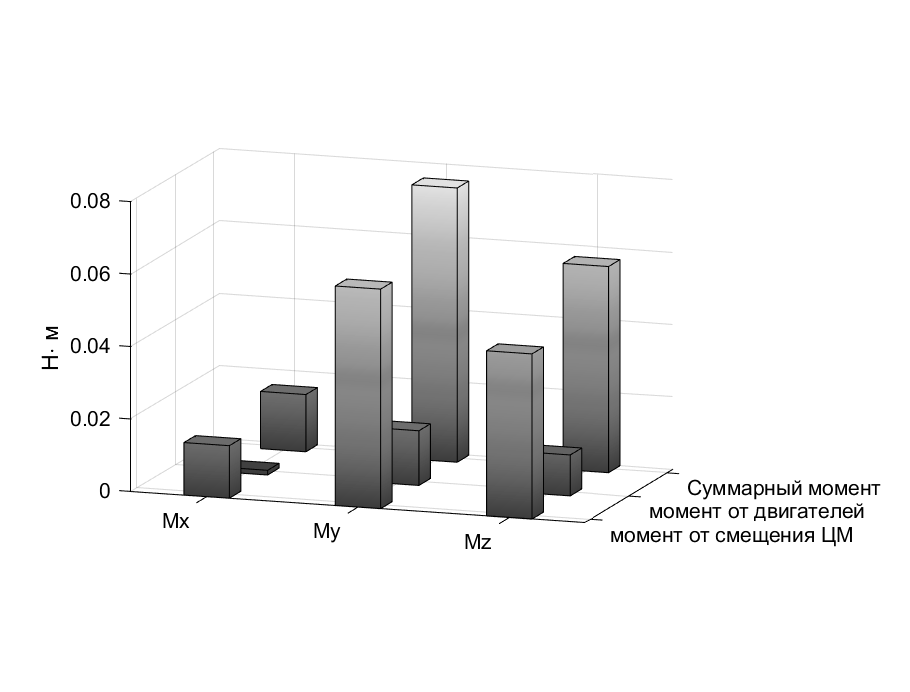
\includegraphics[scale=0.7]{images/moments_chart.eps}}
	
	\caption{Распределение моментов по осям $Mx$, $My$, $Mz$ для различных источников воздействия: смещения центра масс, действия двигателей и их суммарного эффекта}
	\label{fig:momentBars}
\end{figure}

На рисунке ~\cref{fig:momentBars} приведено графическое изображение полученных результатов.

Таким образом, при заданных параметрах основной вклад в реактивные моменты вносит смещение центра карданова подвеса относительно центра масс КА, поэтому при компоновке КА указанное смещение должно быть минимизировано.

Итак, на основании изложенного можно сделать вывод о том, что максимальные реактивные моменты, действующие на основание со стороны редукторных приводов во время их функционирования, для представленного набора исходных данных не превышают величину 0,1 \si{\newton\metre}.  Основной вклад в эти моменты вносят составляющие, возникающие от наличия смещения центра карданова подвеса УПК относительно центра масс КА.

С помощью добавочных колец можно подобрать моменты инерции маховиков с целью уменьшения влияния реактивных моментов на КА.



В таблице \cref{tab:tab_pref} приложения~\cref{app:B4} приведён список рекомендуемых
к использованию стандартных префиксов.

В некоторых ситуациях возникает необходимость отойти от требований ГОСТ по оформлению ссылок на
литературу.
В таком случае можно воспользоваться дополнительными опциями пакета \verb+biblatex+.

Например, в ссылке на книгу~\cite{sobenin_kdv} использование опции \verb+maxnames=4+ позволяет
вывести имена всех четырёх авторов.
По ГОСТ имена последних трёх авторов опускаются.

Кроме того, часто возникают проблемы с транслитерованными инициалами. Некоторые буквы русского
алфавита по правилам транслитерации записываются двумя буквами латинского алфавита (ю-yu, ё-yo и
т.д.).
Такие инициалы \verb+biblatex+ будет сокращать до одной буквы, что неверно.
Поправить его работу можно использовав опцию \verb+giveninits=false+.
Пример использования этой опции можно видеть в ссылке~\cite{initials}.

\section{Формулы}\label{sec:ch1/sec3}

Благодаря пакету \textit{icomma}, \LaTeX~одинаково хорошо воспринимает
в~качестве десятичного разделителя и запятую (\(3,1415\)), и точку (\(3.1415\)).

\subsection{Ненумерованные одиночные формулы}\label{subsec:ch1/sec3/sub1}

Вот так может выглядеть формула, которую необходимо вставить в~строку
по~тексту: \(x \approx \sin x\) при \(x \to 0\).

А вот так выглядит ненумерованная отдельностоящая формула c подстрочными
и надстрочными индексами:
\[
    (x_1+x_2)^2 = x_1^2 + 2 x_1 x_2 + x_2^2
\]

Формула с неопределенным интегралом:
\[
    \int f(\alpha+x)=\sum\beta
\]

При использовании дробей формулы могут получаться очень высокие:
\[
    \frac{1}{\sqrt{2}+
        \displaystyle\frac{1}{\sqrt{2}+
            \displaystyle\frac{1}{\sqrt{2}+\cdots}}}
\]

В формулах можно использовать греческие буквы:
%Все \original... команды заранее, ради этого примера, определены в Dissertation\userstyles.tex
\[
    \alpha\beta\gamma\delta\originalepsilon\epsilon\zeta\eta\theta%
    \vartheta\iota\kappa\varkappa\lambda\mu\nu\xi\pi\varpi\rho\varrho%
    \sigma\varsigma\tau\upsilon\originalphi\phi\chi\psi\omega\Gamma\Delta%
    \Theta\Lambda\Xi\Pi\Sigma\Upsilon\Phi\Psi\Omega
\]
\[%https://texfaq.org/FAQ-boldgreek
    \boldsymbol{\alpha\beta\gamma\delta\originalepsilon\epsilon\zeta\eta%
        \theta\vartheta\iota\kappa\varkappa\lambda\mu\nu\xi\pi\varpi\rho%
        \varrho\sigma\varsigma\tau\upsilon\originalphi\phi\chi\psi\omega\Gamma%
        \Delta\Theta\Lambda\Xi\Pi\Sigma\Upsilon\Phi\Psi\Omega}
\]

Для добавления формул можно использовать пары \verb+$+\dots\verb+$+ и \verb+$$+\dots\verb+$$+,
но~они считаются устаревшими.
Лучше использовать их функциональные аналоги \verb+\(+\dots\verb+\)+ и \verb+\[+\dots\verb+\]+.

\subsection{Ненумерованные многострочные формулы}\label{subsec:ch1/sec3/sub2}

Вот так можно написать две формулы, не нумеруя их, чтобы знаки <<равно>> были
строго друг под другом:
\begin{align}
    f_W & =  \min \left( 1, \max \left( 0, \frac{W_{soil} / W_{max}}{W_{crit}} \right)  \right), \nonumber \\
    f_T & =  \min \left( 1, \max \left( 0, \frac{T_s / T_{melt}}{T_{crit}} \right)  \right), \nonumber
\end{align}

Выровнять систему ещё и по переменной \( x \) можно, используя окружение
\verb|alignedat| из пакета \verb|amsmath|. Вот так:
\[
|x| = \left\{
\begin{alignedat}{2}
     &   & x, \quad & \text{eсли } x\geqslant 0 \\
     & - & x, \quad & \text{eсли } x<0
\end{alignedat}
\right.
\]
Здесь первый амперсанд (в исходном \LaTeX\ описании формулы) означает
выравнивание по~левому краю, второй "--- по~\( x \), а~третий "--- по~слову
<<если>>. Команда \verb|\quad| делает большой горизонтальный пробел.

Ещё вариант:
\[
    |x|=
    \begin{cases}
        \phantom{-}x, \text{если } x \geqslant 0 \\
        -x, \text{если } x<0
    \end{cases}
\]

Кроме того, для  нумерованных формул \verb|alignedat| делает вертикальное
выравнивание номера формулы по центру формулы. Например, выравнивание
компонент вектора:
\begin{equation}
    \label{eq:2p3}
    \begin{alignedat}{2}
        {\mathbf{N}}_{o1n}^{(j)} = \,{\sin} \phi\,n\!\left(n+1\right)
        {\sin}\theta\,
        \pi_n\!\left({\cos} \theta\right)
        \frac{
        z_n^{(j)}\!\left( \rho \right)
        }{\rho}\,
         & {\boldsymbol{\hat{\mathrm e}}}_{r}\,+      \\
        +\,
        {\sin} \phi\,
        \tau_n\!\left({\cos} \theta\right)
        \frac{
        \left[\rho z_n^{(j)}\!\left( \rho \right)\right]^{\prime}
        }{\rho}\,
         & {\boldsymbol{\hat{\mathrm e}}}_{\theta}\,+ \\
        +\,
        {\cos} \phi\,
        \pi_n\!\left({\cos} \theta\right)
        \frac{
        \left[\rho z_n^{(j)}\!\left( \rho \right)\right]^{\prime}
        }{\rho}\,
         & {\boldsymbol{\hat{\mathrm e}}}_{\phi}\:.
    \end{alignedat}
\end{equation}

Ещё об отступах. Иногда для лучшей <<читаемости>> формул полезно
немного исправить стандартные интервалы \LaTeX\ с учётом логической
структуры самой формулы. Например в формуле~\cref{eq:2p3} добавлен
небольшой отступ \verb+\,+ между основными сомножителями, ниже
результат применения всех вариантов отступа:
\begin{align*}
    \backslash!             & \quad f(x) = x^2\! +3x\! +2         \\
    \mbox{по-умолчанию}     & \quad f(x) = x^2+3x+2               \\
    \backslash,             & \quad f(x) = x^2\, +3x\, +2         \\
    \backslash{:}           & \quad f(x) = x^2\: +3x\: +2         \\
    \backslash;             & \quad f(x) = x^2\; +3x\; +2         \\
    \backslash \mbox{space} & \quad f(x) = x^2\ +3x\ +2           \\
    \backslash \mbox{quad}  & \quad f(x) = x^2\quad +3x\quad +2   \\
    \backslash \mbox{qquad} & \quad f(x) = x^2\qquad +3x\qquad +2
\end{align*}

Можно использовать разные математические алфавиты:
\begin{align}
    \mathcal{ABCDEFGHIJKLMNOPQRSTUVWXYZ} \nonumber  \\
    \mathfrak{ABCDEFGHIJKLMNOPQRSTUVWXYZ} \nonumber \\
    \mathbb{ABCDEFGHIJKLMNOPQRSTUVWXYZ} \nonumber
\end{align}

Посмотрим на систему уравнений на примере аттрактора Лоренца:

\[
\left\{
\begin{array}{rl}
    \dot x = & \sigma (y-x)  \\
    \dot y = & x (r - z) - y \\
    \dot z = & xy - bz
\end{array}
\right.
\]

А для вёрстки матриц удобно использовать многоточия:
\[
    \left(
        \begin{array}{ccc}
            a_{11} & \ldots & a_{1n} \\
            \vdots & \ddots & \vdots \\
            a_{n1} & \ldots & a_{nn} \\
        \end{array}
    \right)
\]

\subsection{Нумерованные формулы}\label{subsec:ch1/sec3/sub3}

А вот так пишется нумерованная формула:
\begin{equation}
    \label{eq:equation1}
    e = \lim_{n \to \infty} \left( 1+\frac{1}{n} \right) ^n
\end{equation}

Нумерованных формул может быть несколько:
\begin{equation}
    \label{eq:equation2}
    \lim_{n \to \infty} \sum_{k=1}^n \frac{1}{k^2} = \frac{\pi^2}{6}
\end{equation}

Впоследствии на формулы~\cref{eq:equation1, eq:equation2} можно ссылаться.

Сделать так, чтобы номер формулы стоял напротив средней строки, можно,
используя окружение \verb|multlined| (пакет \verb|mathtools|) вместо
\verb|multline| внутри окружения \verb|equation|. Вот так:
\begin{equation} % \tag{S} % tag - вписывает свой текст
    \label{eq:equation3}
    \begin{multlined}
        1+ 2+3+4+5+6+7+\dots + \\
        + 50+51+52+53+54+55+56+57 + \dots + \\
        + 96+97+98+99+100=5050
    \end{multlined}
\end{equation}

Уравнения~\cref{eq:subeq_1,eq:subeq_2} демонстрируют возможности
окружения \verb|subequations| (пакет \verb|amsmath|).
\begin{subequations}
    \label{eq:subeq_1}
    \begin{gather}
        y = x^2 + 1 \label{eq:subeq_1-1} \\
        y = 2 x^2 - x + 1 \label{eq:subeq_1-2}
    \end{gather}
\end{subequations}
Ссылки на отдельные уравнения~\cref{eq:subeq_1-1,eq:subeq_1-2,eq:subeq_2-1}.
\begin{subequations}
    \label{eq:subeq_2}
    \begin{align}
        y & = x^3 + x^2 + x + 1 \label{eq:subeq_2-1} \\
        y & = x^2
    \end{align}
\end{subequations}

\subsection{Форматирование чисел и размерностей величин}\label{sec:units}

Числа форматируются при помощи команды \verb|\num|:
\num{5,3};
\num{2,3e8};
\num{12345,67890};
\num{2,6 d4};
\num{1+-2i};
\num{.3e45};
\num[exponent-base=2]{5 e64};
\num[exponent-base=2,exponent-to-prefix]{5 e64};
\num{1.654 x 2.34 x 3.430}
\num{1 2 x 3 / 4}.
Для написания последовательности чисел можно использовать команды \verb|\numlist| и \verb|\numrange|:
\numlist{10;30;50;70}; \numrange{10}{30}.
Значения углов можно форматировать при помощи команды \verb|\ang|:
\ang{2.67};
\ang{30,3};
\ang{-1;;};
\ang{;-2;};
\ang{;;-3};
\ang{300;10;1}.

Обратите внимание, что ГОСТ запрещает использование знака <<->> для обозначения отрицательных чисел
за исключением формул, таблиц и~рисунков.
Вместо него следует использовать слово <<минус>>.

Размерности можно записывать при помощи команд \verb|\si| и \verb|\SI|:
\si{\farad\squared\lumen\candela};
\si{\joule\per\mole\per\kelvin};
\si[per-mode = symbol-or-fraction]{\joule\per\mole\per\kelvin};
\si{\metre\per\second\squared};
\SI{0.10(5)}{\neper};
\SI{1.2-3i e5}{\joule\per\mole\per\kelvin};
\SIlist{1;2;3;4}{\tesla};
\SIrange{50}{100}{\volt}.
Список единиц измерений приведён в таблицах~\cref{tab:unit:base,
    tab:unit:derived,tab:unit:accepted,tab:unit:physical,tab:unit:other}.
Приставки единиц приведены в~таблице~\cref{tab:unit:prefix}.

С дополнительными опциями форматирования можно ознакомиться в~описании пакета \texttt{siunitx};
изменить или добавить единицы измерений можно в~файле \texttt{siunitx.cfg}.

\begin{table}
    \centering
    \captionsetup{justification=centering} % выравнивание подписи по-центру
    \caption{Основные величины СИ}\label{tab:unit:base}
    \begin{tabular}{llc}
        \toprule
        Название  & Команда          & Символ         \\
        \midrule
        Ампер     & \verb|\ampere|   & \si{\ampere}   \\
        Кандела   & \verb|\candela|  & \si{\candela}  \\
        Кельвин   & \verb|\kelvin|   & \si{\kelvin}   \\
        Килограмм & \verb|\kilogram| & \si{\kilogram} \\
        Метр      & \verb|\metre|    & \si{\metre}    \\
        Моль      & \verb|\mole|     & \si{\mole}     \\
        Секунда   & \verb|\second|   & \si{\second}   \\
        \bottomrule
    \end{tabular}
\end{table}

\begin{table}
    \small
    \centering
    \begin{threeparttable}% выравнивание подписи по границам таблицы
        \caption{Производные единицы СИ}\label{tab:unit:derived}
        \begin{tabular}{llc|llc}
            \toprule
            Название       & Команда               & Символ              & Название & Команда & Символ \\
            \midrule
            Беккерель      & \verb|\becquerel|     & \si{\becquerel}     &
            Ньютон         & \verb|\newton|        & \si{\newton}                                      \\
            Градус Цельсия & \verb|\degreeCelsius| & \si{\degreeCelsius} &
            Ом             & \verb|\ohm|           & \si{\ohm}                                         \\
            Кулон          & \verb|\coulomb|       & \si{\coulomb}       &
            Паскаль        & \verb|\pascal|        & \si{\pascal}                                      \\
            Фарад          & \verb|\farad|         & \si{\farad}         &
            Радиан         & \verb|\radian|        & \si{\radian}                                      \\
            Грей           & \verb|\gray|          & \si{\gray}          &
            Сименс         & \verb|\siemens|       & \si{\siemens}                                     \\
            Герц           & \verb|\hertz|         & \si{\hertz}         &
            Зиверт         & \verb|\sievert|       & \si{\sievert}                                     \\
            Генри          & \verb|\henry|         & \si{\henry}         &
            Стерадиан      & \verb|\steradian|     & \si{\steradian}                                   \\
            Джоуль         & \verb|\joule|         & \si{\joule}         &
            Тесла          & \verb|\tesla|         & \si{\tesla}                                       \\
            Катал          & \verb|\katal|         & \si{\katal}         &
            Вольт          & \verb|\volt|          & \si{\volt}                                        \\
            Люмен          & \verb|\lumen|         & \si{\lumen}         &
            Ватт           & \verb|\watt|          & \si{\watt}                                        \\
            Люкс           & \verb|\lux|           & \si{\lux}           &
            Вебер          & \verb|\weber|         & \si{\weber}                                       \\
            \bottomrule
        \end{tabular}
    \end{threeparttable}
\end{table}

\begin{table}
    \centering
    \begin{threeparttable}% выравнивание подписи по границам таблицы
        \caption{Внесистемные единицы}\label{tab:unit:accepted}

        \begin{tabular}{llc}
            \toprule
            Название        & Команда           & Символ          \\
            \midrule
            День            & \verb|\day|       & \si{\day}       \\
            Градус          & \verb|\degree|    & \si{\degree}    \\
            Гектар          & \verb|\hectare|   & \si{\hectare}   \\
            Час             & \verb|\hour|      & \si{\hour}      \\
            Литр            & \verb|\litre|     & \si{\litre}     \\
            Угловая минута  & \verb|\arcminute| & \si{\arcminute} \\
            Угловая секунда & \verb|\arcsecond| & \si{\arcsecond} \\ %
            Минута          & \verb|\minute|    & \si{\minute}    \\
            Тонна           & \verb|\tonne|     & \si{\tonne}     \\
            \bottomrule
        \end{tabular}
    \end{threeparttable}
\end{table}

\begin{table}
    \centering
    \captionsetup{justification=centering}
    \caption{Внесистемные единицы, получаемые из эксперимента}\label{tab:unit:physical}
    \begin{tabular}{llc}
        \toprule
        Название                & Команда                  & Символ                 \\
        \midrule
        Астрономическая единица & \verb|\astronomicalunit| & \si{\astronomicalunit} \\
        Атомная единица массы   & \verb|\atomicmassunit|   & \si{\atomicmassunit}   \\
        Боровский радиус        & \verb|\bohr|             & \si{\bohr}             \\
        Скорость света          & \verb|\clight|           & \si{\clight}           \\
        Дальтон                 & \verb|\dalton|           & \si{\dalton}           \\
        Масса электрона         & \verb|\electronmass|     & \si{\electronmass}     \\
        Электрон Вольт          & \verb|\electronvolt|     & \si{\electronvolt}     \\
        Элементарный заряд      & \verb|\elementarycharge| & \si{\elementarycharge} \\
        Энергия Хартри          & \verb|\hartree|          & \si{\hartree}          \\
        Постоянная Планка       & \verb|\planckbar|        & \si{\planckbar}        \\
        \bottomrule
    \end{tabular}
\end{table}

\begin{table}
    \centering
    \begin{threeparttable}% выравнивание подписи по границам таблицы
        \caption{Другие внесистемные единицы}\label{tab:unit:other}
        \begin{tabular}{llc}
            \toprule
            Название                  & Команда              & Символ             \\
            \midrule
            Ангстрем                  & \verb|\angstrom|     & \si{\angstrom}     \\
            Бар                       & \verb|\bar|          & \si{\bar}          \\
            Барн                      & \verb|\barn|         & \si{\barn}         \\
            Бел                       & \verb|\bel|          & \si{\bel}          \\
            Децибел                   & \verb|\decibel|      & \si{\decibel}      \\
            Узел                      & \verb|\knot|         & \si{\knot}         \\
            Миллиметр ртутного столба & \verb|\mmHg|         & \si{\mmHg}         \\
            Морская миля              & \verb|\nauticalmile| & \si{\nauticalmile} \\
            Непер                     & \verb|\neper|        & \si{\neper}        \\
            \bottomrule
        \end{tabular}
    \end{threeparttable}
\end{table}

\begin{table}
    \small
    \centering
    \begin{threeparttable}% выравнивание подписи по границам таблицы
        \caption{Приставки СИ}\label{tab:unit:prefix}
        \begin{tabular}{llcc|llcc}
            \toprule
            Приставка & Команда       & Символ      & Степень      &
            Приставка & Команда       & Символ      & Степень        \\
            \midrule
            Иокто     & \verb|\yocto| & \si{\yocto} & \textminus24 &
            Дека      & \verb|\deca|  & \si{\deca}  & 1              \\
            Зепто     & \verb|\zepto| & \si{\zepto} & \textminus21 &
            Гекто     & \verb|\hecto| & \si{\hecto} & 2              \\
            Атто      & \verb|\atto|  & \si{\atto}  & \textminus18 &
            Кило      & \verb|\kilo|  & \si{\kilo}  & 3              \\
            Фемто     & \verb|\femto| & \si{\femto} & \textminus15 &
            Мега      & \verb|\mega|  & \si{\mega}  & 6              \\
            Пико      & \verb|\pico|  & \si{\pico}  & \textminus12 &
            Гига      & \verb|\giga|  & \si{\giga}  & 9              \\
            Нано      & \verb|\nano|  & \si{\nano}  & \textminus9  &
            Терра     & \verb|\tera|  & \si{\tera}  & 12             \\
            Микро     & \verb|\micro| & \si{\micro} & \textminus6  &
            Пета      & \verb|\peta|  & \si{\peta}  & 15             \\
            Милли     & \verb|\milli| & \si{\milli} & \textminus3  &
            Екса      & \verb|\exa|   & \si{\exa}   & 18             \\
            Санти     & \verb|\centi| & \si{\centi} & \textminus2  &
            Зетта     & \verb|\zetta| & \si{\zetta} & 21             \\
            Деци      & \verb|\deci|  & \si{\deci}  & \textminus1  &
            Иотта     & \verb|\yotta| & \si{\yotta} & 24             \\
            \bottomrule
        \end{tabular}
    \end{threeparttable}
\end{table}

\subsection{Заголовки с формулами: \texorpdfstring{\(a^2 + b^2 = c^2\)}{%
        a\texttwosuperior\ + b\texttwosuperior\ = c\texttwosuperior},
    \texorpdfstring{\(\left\vert\textrm{{Im}}\Sigma\left(
            \protect\varepsilon\right)\right\vert\approx const\)}{|ImΣ (ε)| ≈ const},
    \texorpdfstring{\(\sigma_{xx}^{(1)}\)}{σ\_\{xx\}\textasciicircum\{(1)\}}
}\label{subsec:with_math}

Пакет \texttt{hyperref} берёт текст для закладок в pdf-файле из~аргументов
команд типа \verb|\section|, которые могут содержать математические формулы,
а~также изменения цвета текста или шрифта, которые не отображаются в~закладках.
Чтобы использование формул в заголовках не вызывало в~логе компиляции появление
предупреждений типа <<\texttt{Token not allowed in~a~PDF string
    (Unicode):(hyperref) removing...}>>, следует использовать конструкцию
\verb|\texorpdfstring{}{}|, где в~первых фигурных скобках указывается
формула, а~во~вторых "--- запись формулы для закладок.

\section{Рецензирование текста}\label{sec:markup}

В шаблоне для диссертации и автореферата заданы команды рецензирования.
Они видны при компиляции шаблона в режиме черновика или при установке
соответствующей настройки (\verb+showmarkup+) в~файле \verb+common/setup.tex+.

Команда \verb+\todo+ отмечает текст красным цветом.
\todo{Например, так.}

Команда \verb+\note+ позволяет выбрать цвет текста.
\note{Чёрный, } \note[red]{красный, } \note[green]{зелёный, }
\note[blue]{синий.} \note[orange]{Обратите внимание на ширину и расстановку
    формирующихся пробелов, в~результате приведённой записи (зависит также
    от~применяемого компилятора).}

Окружение \verb+commentbox+ также позволяет выбрать цвет.

\begin{commentbox}[red]
    Красный текст.

    Несколько параграфов красного текста.
\end{commentbox}

\begin{commentbox}[blue]
    Синяя формула.

    \begin{equation}
        \alpha + \beta = \gamma
    \end{equation}
\end{commentbox}

\verb+commentbox+ позволяет закомментировать участок кода в~режиме чистовика.
Чтобы убрать кусок кода для всех режимов, можно использовать окружение
\verb+comment+.

\begin{comment}
Этот текст всегда скрыт.
\end{comment}

\section{Работа со списком сокращений и~условных обозначений}\label{sec:acronyms}

С помощью пакета \texttt{nomencl} можно создавать удобный сортированный список
сокращений и условных обозначений во время написания текста. Вызов
\verb+\nomenclature+ добавляет нужный символ или сокращение с~описанием
в~список, который затем печатается вызовом \verb+\printnomenclature+
в~соответствующем разделе.
Для того, чтобы эти операции прошли, потребуется дополнительный вызов
\verb+makeindex -s nomencl.ist -o %.nls %.nlo+ в~командной строке, где вместо
\verb+%+ следует подставить имя главного файла проекта (\verb+dissertation+
для этого шаблона).
Затем потребуется один или два дополнительных вызова компилятора проекта.
\begin{equation}
    \omega = c k,
\end{equation}
где \( \omega \) "--- частота света, \( c \) "--- скорость света, \( k \) "---модуль волнового вектора.
\nomenclature{\(\omega\)}{частота света\nomrefeq}
\nomenclature{\(c\)}{скорость света\nomrefpage}
\nomenclature{\(k\)}{модуль волнового вектора\nomrefeqpage}
Использование
\begin{verbatim}
\nomenclature{\(\omega\)}{частота света\nomrefeq}
\nomenclature{\(c\)}{скорость света\nomrefpage}
\nomenclature{\(k\)}{модуль волнового вектора\nomrefeqpage}
\end{verbatim}
после уравнения добавит в список условных обозначений три записи.
Ссылки \verb+\nomrefeq+ на последнее уравнение, \verb+\nomrefpage+ "--- на
страницу, \verb+\nomrefeqpage+ "--- сразу на~последнее уравнение и~на~страницу,
можно опускать и~не~использовать.

Группировкой и сортировкой пунктов в списке можно управлять с~помощью указания
дополнительных аргументов к команде \verb+nomenclature+.
Например, при вызове
\begin{verbatim}
\nomenclature[03]{\( \hbar \)}{постоянная Планка}
\nomenclature[01]{\( G \)}{гравитационная постоянная}
\end{verbatim}
\( G \) будет стоять в списке выше, чем \( \hbar \).
Для корректных вертикальных отступов между строками в описании лучше
не~использовать многострочные формулы в~списке обозначений.

\nomenclature{%
    \( \begin{rcases}
        a_n \\
        b_n
    \end{rcases} \)%
}{коэффициенты разложения Ми в дальнем поле соответствующие электрическим и
    магнитным мультиполям}
\nomenclature[a\( e \)]{\( {\boldsymbol{\hat{\mathrm e}}} \)}{единичный вектор}
\nomenclature{\( E_0 \)}{амплитуда падающего поля}
\nomenclature{\( j \)}{тип функции Бесселя}
\nomenclature{\( k \)}{волновой вектор падающей волны}
\nomenclature{%
    \( \begin{rcases}
        a_n \\
        b_n
    \end{rcases} \)%
}{и снова коэффициенты разложения Ми в дальнем поле соответствующие
    электрическим и магнитным мультиполям. Добавлено много текста, так что
    описание группы условных обозначений значительно превысило высоту этой
    группы...}
\nomenclature{\( L \)}{общее число слоёв}
\nomenclature{\( l \)}{номер слоя внутри стратифицированной сферы}
\nomenclature{\( \lambda \)}{длина волны электромагнитного излучения в вакууме}
\nomenclature{\( n \)}{порядок мультиполя}
\nomenclature{%
    \( \begin{rcases}
        {\mathbf{N}}_{e1n}^{(j)} & {\mathbf{N}}_{o1n}^{(j)} \\
        {\mathbf{M}_{o1n}^{(j)}} & {\mathbf{M}_{e1n}^{(j)}}
    \end{rcases} \)%
}{сферические векторные гармоники}
\nomenclature{\( \mu \)}{магнитная проницаемость в вакууме}
\nomenclature{\( r, \theta, \phi \)}{полярные координаты}
\nomenclature{\( \omega \)}{частота падающей волны}

С помощью \verb+nomenclature+ можно включать в~список сокращения,
не~используя их~в~тексте.
% запись сокращения в список происходит командой \nomenclature,
% а не употреблением самого сокращения
\nomenclature{FEM}{finite element method, метод конечных элементов}
\nomenclature{FIT}{finite integration technique, метод конечных интегралов}
\nomenclature{FMM}{fast multipole method, быстрый метод многополюсника}
\nomenclature{FVTD}{finite volume time-domain, метод конечных объёмов
    во~временной области}
\nomenclature{MLFMA}{multilevel fast multipole algorithm, многоуровневый
    быстрый алгоритм многополюсника}
\nomenclature{BEM}{boundary element method, метод граничных элементов}
\nomenclature{CST MWS}{Computer Simulation Technology Microwave Studio
    программа для компьютерного моделирования уравнен Максвелла}
\nomenclature{DDA}{discrete dipole approximation, приближение дискретиных
    диполей}
\nomenclature{FDFD}{finite difference frequency domain, метод конечных
    разностей в~частотной области}
\nomenclature{FDTD}{finite difference time domain, метод конечных разностей
    во~временной области}
\nomenclature{MoM}{method of moments, метод моментов}
\nomenclature{MSTM}{multiple sphere T-Matrix, метод Т-матриц для множества
    сфер}
\nomenclature{PSTD}{pseudospectral time domain method, псевдоспектральный метод
    во~временной области}
\nomenclature{TLM}{transmission line matrix method, метод матриц линий передач}

\FloatBarrier
